\subsubsection{GSS\cite{gou_fast_2018}}

\paragraph{}
GSS is the latest graph summarization technique that has been introduced up to date which was published in 2018. Even when using 1/256 memory size of the state of the art graph summarization algorithm, GSS still significantly outperformed it for most queries. The GSS paper points out that even if TCM and gMatrix support all queries in the streaming graphs in contrast to CM sketches\cite{cormode_improved_2003} and gSketch which only supports queries for edges and do not get involved with the topology of the underlying graph, they suffer from poor accuracy. GSS improves upon TCM and gMatrix to increase the accuracy with less memory usage.

\paragraph{}
GSS defines three graph primitives as,

\begin{itemize}
    \item Edge query
    \item 1-hop Successor query
    \item 1-hop Precursor query
\end{itemize}

\paragraph{}
By supporting all these 3 types of queries it is possible to reconstruct the entire graph. Therefore it is also possible to run any kind of query against a sketch which supports all 3 of the above primitives.

\paragraph{}
The intuition behind the basic version of the GSS can be illustrated as below.

\begin{figure}[H]
    \centering 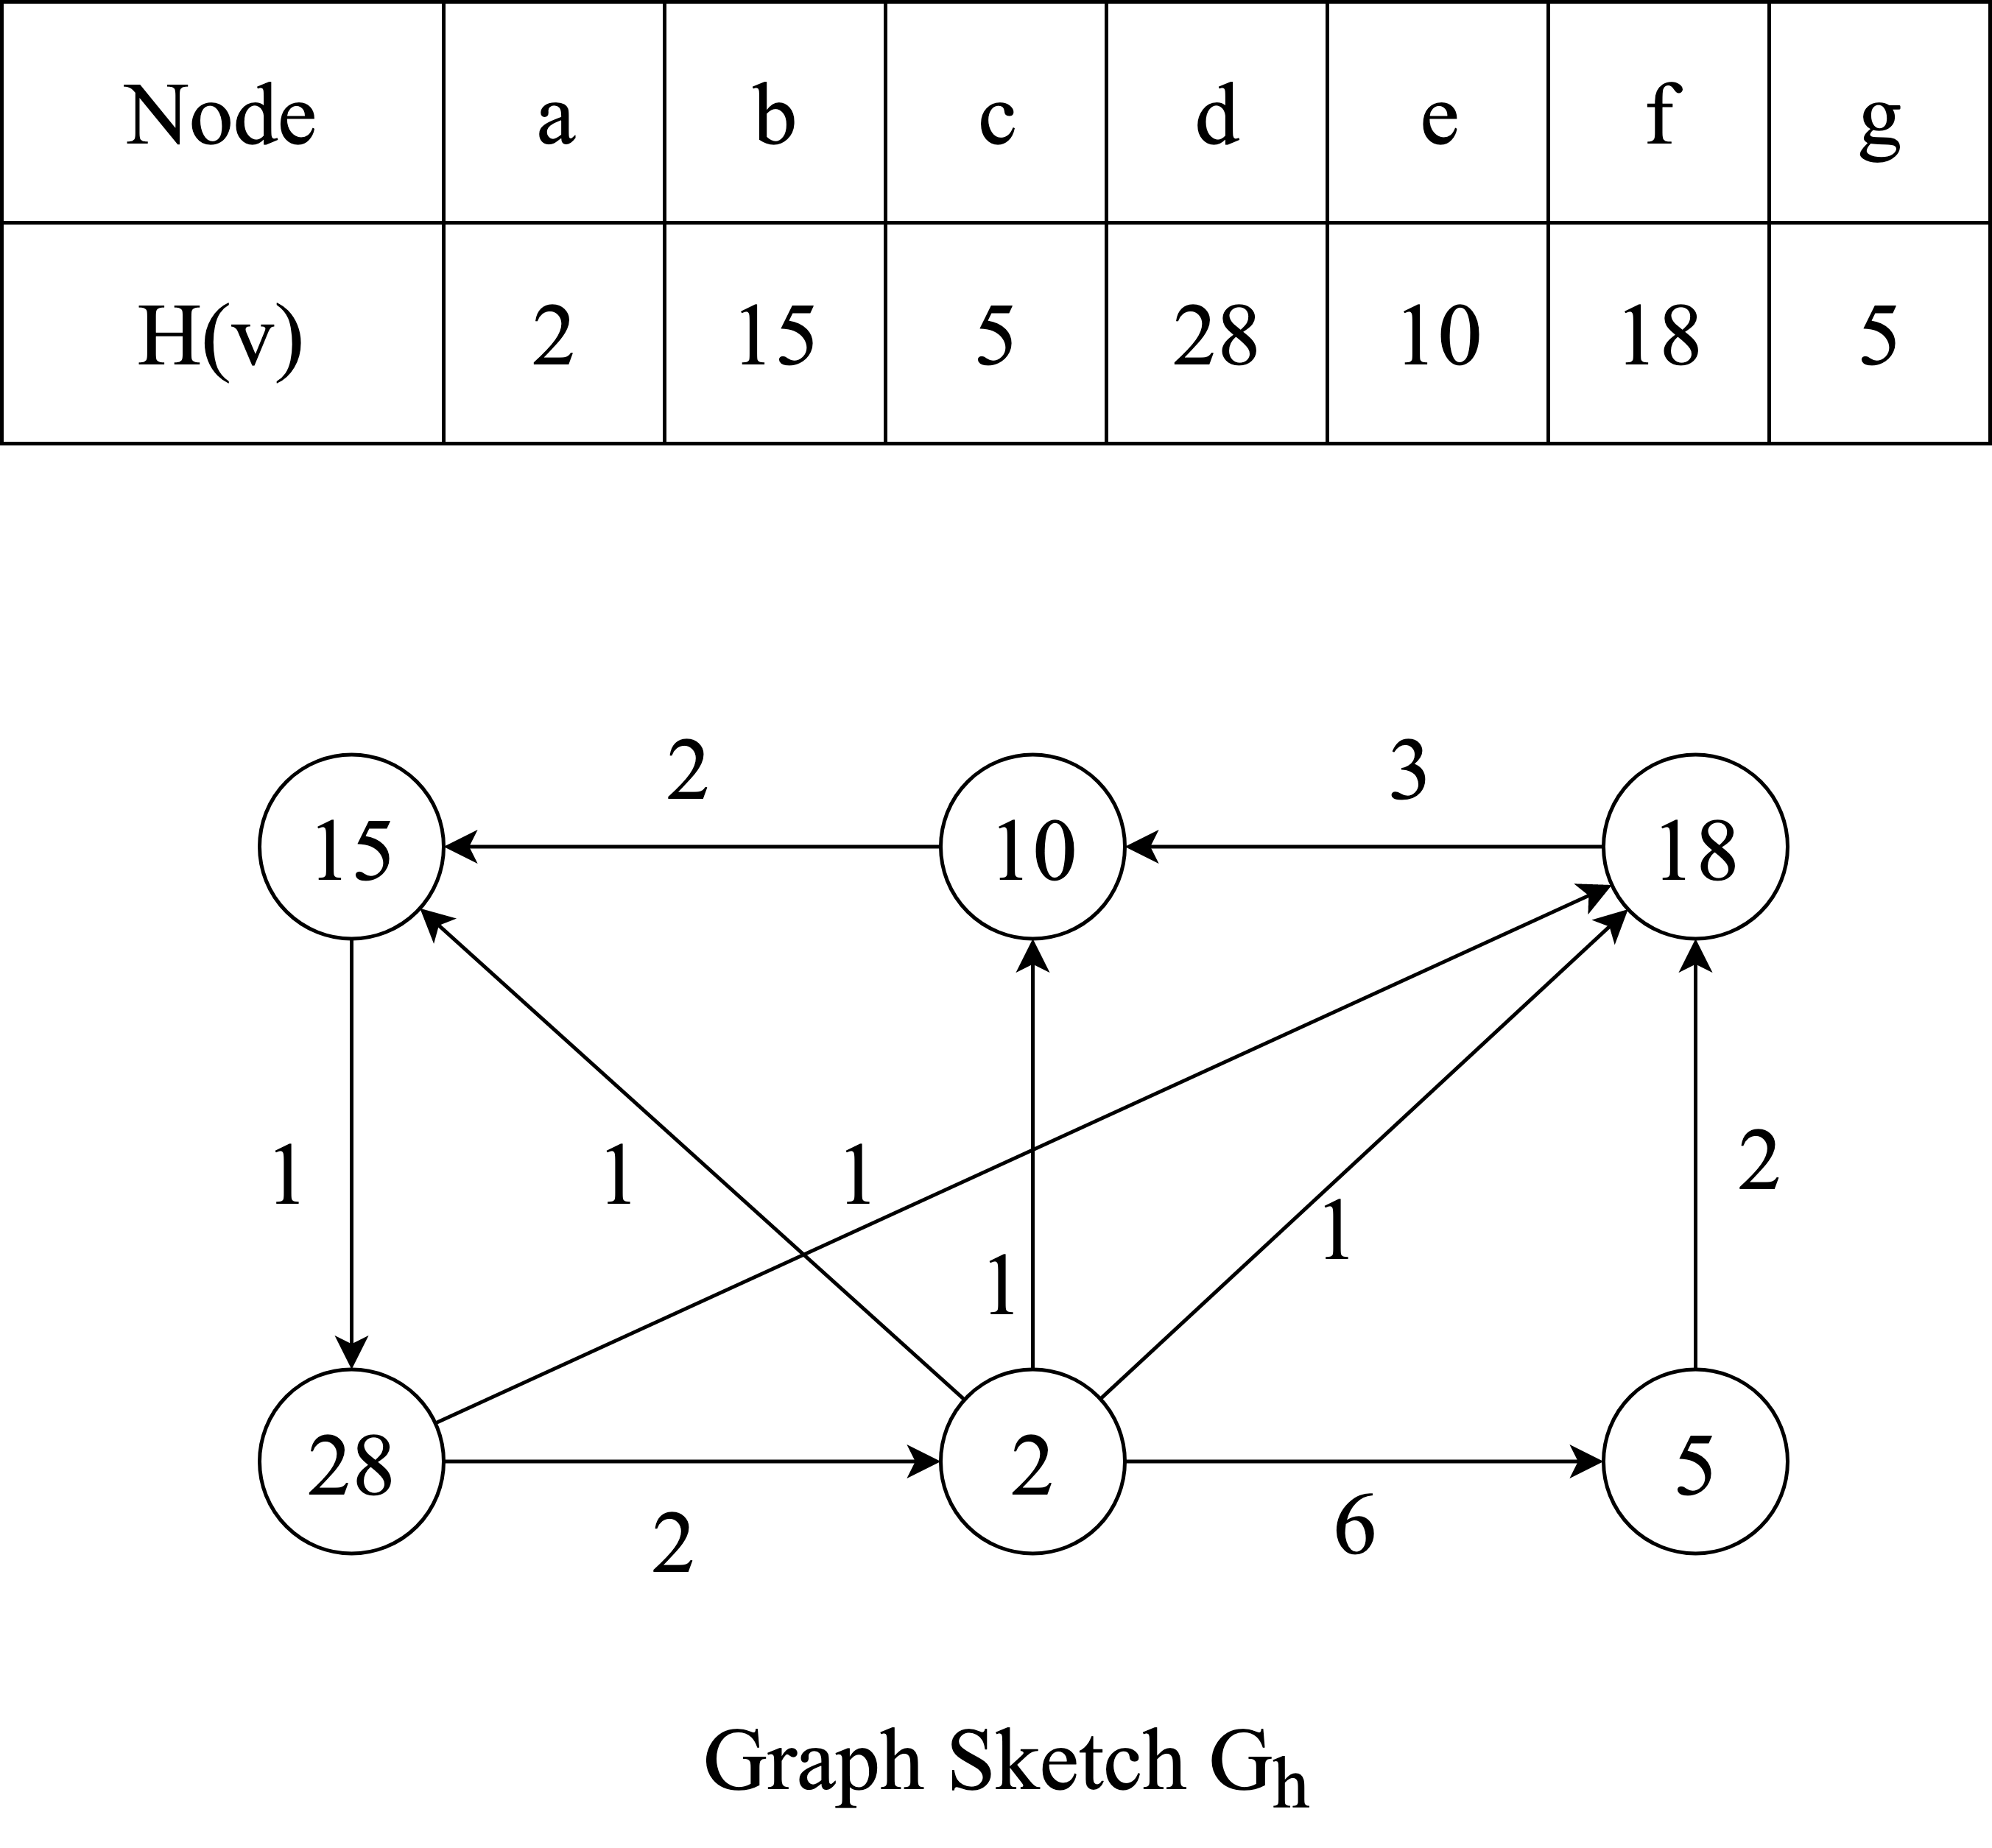
\includegraphics[width=0.6\textwidth]{gss1}
    \caption{A sample map function\cite{gou_fast_2018}}
    \label{fig:gss1}
\end{figure}

\paragraph{}
\(H(.)\) is a hash function which is used on the vertices of the original graph stream to create the graph sketch \(G\textsubscript{h}\) as indicated in Figure \ref{fig:gss1}.

\paragraph{}
A GSS sketch consists of two parts,

\begin{enumerate}
    \item Adjacency matrix
    \item List buffer B for leftover edges
\end{enumerate}

\paragraph{}
For each node in the sketch graph \(G\textsubscript{h}\), an address \(h(v)\) and a fingerprint \(f(v)\) is defined. Each edge \(H(s)\), \(H(d)\) is mapped into a bucket in the row \(h(s)\), column \(h(d)\) of the matrix. \([\langle f(s), f(d)\rangle, w]\) is recorded in the corresponding bucket of the matrix, where \(w\) is the edge weight and \(f(s)\), \(f(d)\) are the fingerprints for the source and destination. This can be seen in the sample of GSS sketch shown in Figure \ref{fig:gss2}.

\begin{figure}[H]
    \centering
    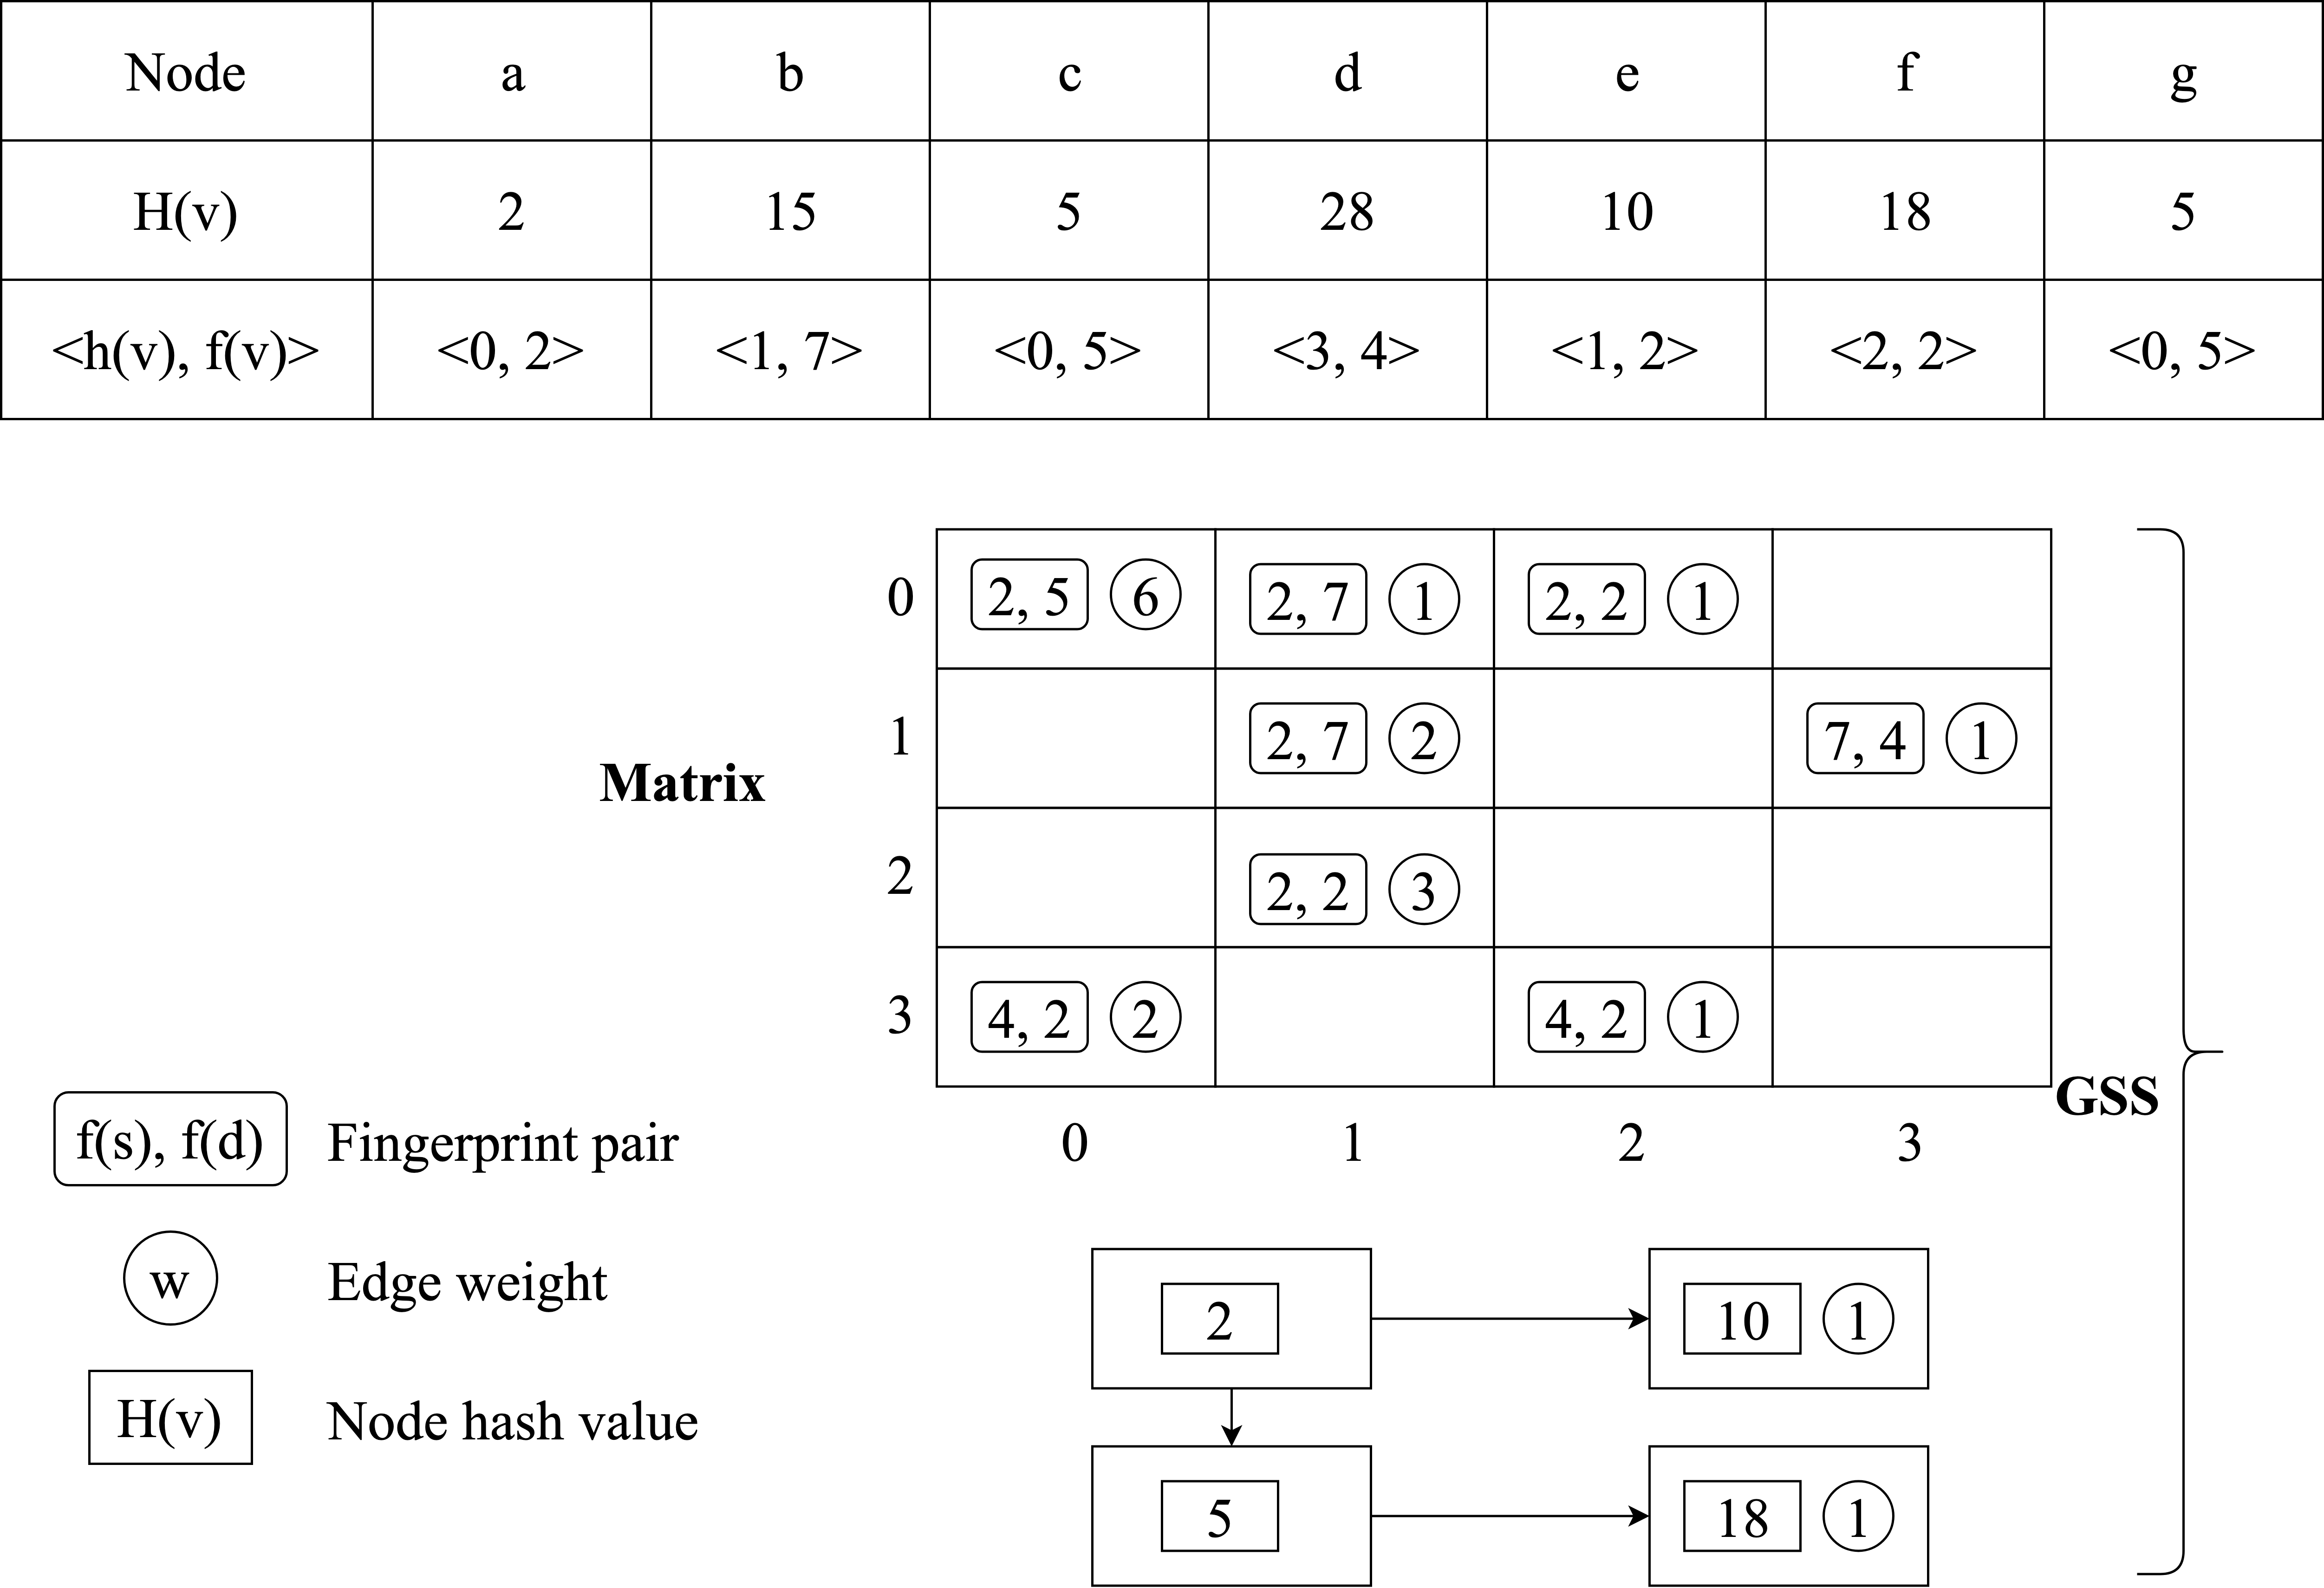
\includegraphics[width=\textwidth]{gss2}
    \caption{A sample version of the basic data structure\cite{gou_fast_2018}}
    \label{fig:gss2}
\end{figure}